\documentclass{article}


% if you need to pass options to natbib, use, e.g.:
%     \PassOptionsToPackage{numbers, compress}{natbib}
% before loading neurips_2023


% ready for submission
\usepackage[final]{neurips_2023}


\usepackage[utf8]{inputenc} % allow utf-8 input
\usepackage[T1]{fontenc}    % use 8-bit T1 fonts
\usepackage{hyperref}       % hyperlinks
\usepackage{url}            % simple URL typesetting
\usepackage{booktabs}       % professional-quality tables
\usepackage{amsfonts}       % blackboard math symbols
\usepackage{nicefrac}       % compact symbols for 1/2, etc.
\usepackage{microtype}      % microtypography
\usepackage{xcolor}         % colors

\usepackage{float}          % table float placement
\usepackage{graphicx}       % figures
\usepackage{amsmath}

\usepackage{enumitem}       % customized lists


\title{Knowledge Distillation with Adaptive Sampling\\for Mathematical Reasoning}


\author{
  Zhang Entong
}


\begin{document}


\maketitle


\begin{abstract}
Large language models (LLMs) have demonstrated remarkable capabilities in mathematical reasoning, yet their computational requirements pose challenges for practical deployment. In this paper, we investigate chain-of-thought (CoT) knowledge distillation for mathematical reasoning, using DeepSeek-R1-Distill-Qwen-1.5B as the teacher and Qwen2.5-0.5B as the student. We compare multiple strategies for constructing CoT training data on GSM8K and MATH benchmarks, and identify a \textit{distillation tax}: fine-tuning instruction-tuned models on foreign-style CoT traces degrades their native reasoning. Switching to a base model eliminates this confound, yielding improvements unambiguously attributable to distillation. We further demonstrate that semantic deduplication is critical for preventing template overfitting while preserving problem coverage, and that multi-temperature generation provides meaningfully diverse reasoning paths that single-temperature multi-sampling cannot replicate.
\end{abstract}


\section{Introduction}

\subsection{Background}

Large language models (LLMs) have achieved significant breakthroughs in natural language processing, demonstrating impressive capabilities across a wide range of tasks including text generation, code synthesis, and mathematical reasoning. Recent advances, exemplified by models such as DeepSeek-R1~\cite{deepseek2025r1}, have shown that scaling model size and training data, combined with reinforcement learning, leads to emergent reasoning abilities. However, the deployment of these large models in resource-constrained environments-such as mobile devices, edge computing platforms, and real-time applications-remains challenging due to their substantial computational and memory requirements.

Mathematical reasoning presents a particularly demanding challenge for language models, requiring multi-step logical deduction, symbolic manipulation, and numerical computation. Benchmarks such as GSM8K and MATH have been widely adopted to evaluate the mathematical reasoning capabilities of LLMs. While large models achieve high accuracy on these benchmarks, smaller models often struggle with complex multi-step reasoning, creating a significant performance gap.

\subsection{Motivation}

Knowledge distillation provides a principled framework for transferring knowledge from a large, capable teacher model to a smaller, more efficient student model. In the context of mathematical reasoning, the teacher model can generate high-quality chain-of-thought reasoning traces, which serve as supervised training data for the student model. This approach, known as CoT distillation~\cite{ho2023large}, has been shown to be effective in improving the reasoning capabilities of smaller models.

However, a key challenge in CoT distillation is the quality and diversity of the generated training data. Single-temperature generation may either lack diversity (at low temperatures) or produce noisy, incorrect reasoning traces (at high temperatures). Furthermore, the choice of sampling strategy directly impacts the coverage of correct solutions and the efficiency of the distillation pipeline.

In this work, we address these challenges by exploring multiple CoT generation strategies—including multi-temperature sampling with semantic deduplication and confidence-guided adaptive sampling—and comparing their effects on training data quality, diversity, and downstream student performance on GSM8K and MATH benchmarks.

\section{Related Work}

\subsection{Knowledge Distillation for Reasoning}

Knowledge distillation trains a compact student model to mimic the output distribution of a larger teacher model by minimizing the Kullback-Leibler divergence between their softened probability distributions. In the context of language models, recent work has demonstrated that large language models can serve as effective reasoning teachers~\cite{ho2023large}, generating high-quality chain-of-thought (CoT) reasoning traces that encode the step-by-step problem-solving process. These CoT traces serve as rich supervision signals for training smaller student models, enabling them to acquire reasoning capabilities that would be difficult to learn from final answers alone.

\subsection{Large Language Models for Mathematical Reasoning}

Recent advances in large language models have significantly pushed the boundaries of mathematical reasoning. DeepSeek-R1~\cite{deepseek2025r1} demonstrates that reinforcement learning can effectively incentivize reasoning capabilities in LLMs, producing models that generate detailed chain-of-thought reasoning traces. These reasoning traces are particularly valuable for knowledge distillation, as they reveal the intermediate steps and logical deductions that lead to correct answers. However, deploying such large models directly is computationally expensive, motivating the use of distillation to transfer their reasoning capabilities into smaller, more efficient models.

\section{Method}

\subsection{Overview}

Our knowledge distillation pipeline consists of four main stages, as illustrated in Figure~\ref{fig:pipeline}: (1) CoT generation using the teacher model, (2) answer extraction and correctness filtering, (3) dataset construction through merging and optional deduplication, and (4) supervised fine-tuning of the student model.

\begin{figure}[H]
    \centering
    \fbox{%
    \begin{minipage}{0.9\textwidth}
    \vspace{4mm}
    \begin{center}
    \textbf{Teacher CoT Generation} $\rightarrow$ \textbf{Answer Filtering} $\rightarrow$ \textbf{Dataset Construction} $\rightarrow$ \textbf{Student Fine-tuning}
    \end{center}
    \vspace{2mm}
    \small
    \begin{itemize}[leftmargin=*]
        \item \textbf{Stage 1:} DeepSeek-R1-Distill-Qwen-1.5B generates CoT reasoning traces via vLLM using one of three strategies: single-temperature, double-temperature, or adaptive sampling
        \item \textbf{Stage 2:} Extract final answers from CoT traces using \texttt{\textbackslash{}boxed\{\}} matching; compare with ground-truth; classify as correct/incorrect/empty
        \item \textbf{Stage 3:} Merge GSM8K and MATH correct samples; optionally deduplicate via sentence-transformers semantic similarity; shuffle
        \item \textbf{Stage 4:} Fine-tune Qwen2.5-0.5B (Instruct initially, then Base) via SFT with label masking on assistant tokens only
    \end{itemize}
    \vspace{2mm}
    \end{minipage}
    }
    \caption{Overview of the knowledge distillation pipeline.}
    \label{fig:pipeline}
\end{figure}

\subsection{Teacher-Student Configuration}

We employ DeepSeek-R1-Distill-Qwen-1.5B as the teacher. Its outputs contain \verb|<think>| tags which are stripped during preprocessing. For the student, we initially used Qwen2.5-0.5B-Instruct but switched to the base model Qwen2.5-0.5B. The Instruct variant already possesses mathematical reasoning capability from instruction tuning, confounding the attribution of distillation gains. The base model has no prior math-specific training, and its pre-training with \verb|<|im\_start|>| tokens enables native chat template support. Both variants use the same format: system prompt, user problem, and assistant CoT answer, with label masking on prompt tokens.

\subsection{CoT Generation Strategies}

We employ three distinct strategies for generating chain-of-thought reasoning traces from the teacher model, each representing a different trade-off between data quality, diversity, and computational cost. All strategies share the same teacher model (DeepSeek-R1-Distill-Qwen-1.5B), the same prompt template (system prompt instructing step-by-step reasoning with final answer in \texttt{\textbackslash{}boxed\{\}}), and the same vLLM-based inference backend.

\subsubsection{Strategy 1: Single-Temperature Generation}

The simplest approach: for each problem in the training set, the teacher generates exactly one CoT reasoning trace at a fixed temperature $T = 0.6$. This temperature provides a moderate level of stochasticity, balancing coherent reasoning against some diversity in solution paths. After generation, each CoT trace undergoes answer extraction, cleaning, and correctness comparison with the ground truth. Only correctly answered traces are retained for student training. This strategy produces the simplest training dataset, used as a reference point for evaluating the more sophisticated strategies that follow.

\subsubsection{Strategy 2: Double-Temperature Generation with Semantic Deduplication}

To increase answer diversity and problem coverage, we generate two CoT traces per problem: one at low temperature ($T = 0.6$) for quality and one at high temperature ($T = 0.9$) for diversity. However, not all high-temperature generations produce meaningfully different answers-many are near-duplicates of the low-temperature counterpart.

To address this, we apply semantic deduplication using Sentence-BERT (\texttt{all-MiniLM-L6-v2}). For each problem, the two generated answers are encoded into 384-dimensional normalized embedding vectors, and their cosine similarity is computed. If the similarity exceeds a threshold of $0.92$, the two answers are considered semantically equivalent and only the low-temperature (higher-quality) version is retained. Otherwise, both answers are kept. This approach balances the diversity benefits of multi-temperature sampling against training set redundancy, yielding a moderately expanded dataset with minimal duplication.

\subsubsection{Strategy 3: Adaptive Sampling with Log-Probability Confidence}

The double-temperature strategy generates multiple samples for all problems indiscriminately, regardless of whether the teacher is already confident in its answer. Our adaptive sampling strategy aims to allocate the extra sampling budget only to problems where the teacher exhibits uncertainty, using per-token log-probability as a lightweight confidence signal.

For each problem, we generate $n = 3$ samples at $T_{\text{low}} = 0.3$ and compute the per-token average log-probability $\bar{\ell}_i = \frac{1}{L}\sum_{t=1}^{L} \log P(y_t|y_{<t}, p)$ for each. The maximum across samples serves as the confidence score; if it exceeds $\tau$, all samples are kept. Otherwise, iterative rounds at $T_{\text{high}} = 0.9$ add 2 samples per round (up to 4 rounds) until the threshold is met. The key advantage over self-consistency voting is zero additional inference cost: vLLM's \texttt{SamplingParams(logprobs=1)} returns log-probabilities natively alongside generated tokens.

\subsubsection{Threshold Calibration Discussion}

In our experiments, $\tau = -1.8$ resulted in 100\% first-round high-confidence classification, including for problems where the teacher produced incorrect answers, indicating the threshold was too lenient. We outline two directions for improving the sampling strategy:

\textbf{1. Static Threshold Calibration.} A simple improvement is to calibrate $\tau$ via a pilot study on a small subset (100--200 problems), examining the log-probability distributions of correct vs.\ incorrect answers to find a more discriminative separation point.

\textbf{2. Learned Sampling Policy.} A more principled approach replaces the fixed temperature-and-count schedule with a learned policy. The decision of whether to continue sampling, and at what temperature, is conditioned on a richer state representation: the problem's semantic embedding (capturing inherent difficulty), the number of samples already generated, the mean and variance of the existing answers' log-probabilities, and whether any answer has already been verified as correct. A lightweight policy network-trained via reinforcement learning with a reward that balances answer coverage against sampling cost-learns to allocate the teacher's generation budget adaptively per problem: stopping early for trivially easy problems, escalating to high-temperature exploration only when low-temperature samples show inconsistent or low-confidence reasoning, and abandoning hopeless cases where additional sampling is unlikely to help.

\subsection{Answer Extraction and Filtering}

After generating CoT traces, we extract final answers using a multi-level matching strategy:
\begin{enumerate}[leftmargin=*]
    \item \textbf{Primary:} Extract content within balanced-brace \texttt{\textbackslash{}boxed\{\}} expressions
    \item \textbf{Fallback 1:} Match the \verb|**Answer:**| marker pattern
    \item \textbf{Fallback 2:} For GSM8K only, extract the last numerical value if the text ends with a period
\end{enumerate}

Extracted answers are cleaned by removing LaTeX formatting commands, units, and unnecessary commas. For GSM8K, correctness is determined by numerical comparison with a tolerance of $10^{-9}$. For MATH, string comparison is used to preserve LaTeX expressions, fractions, and special mathematical notation.

\subsection{CoT Quality Analysis}

Beyond correctness filtering, we analyzed CoT trace quality across all four training datasets for patterns that may negatively impact student training. We define five categories: (1) \textbf{Self-Correction and Hesitation} (markers: ``wait'', ``Oops'', ``Actually,'', ``Hmm'', ``I made a mistake''), where the teacher revises mid-reasoning, creating ambiguous training signals; (2) \textbf{High Line Repetition} ($\geq 4$ identical lines), encouraging verbose exhaustive-search habits; (3) \textbf{Missing \texttt{\textbackslash{}boxed\{\}}} format, using \texttt{**Answer:**} or plain text instead; (4) \textbf{Extreme Length} ($<$200 or $>$3,000 characters); and (5) \textbf{Formatting Artifacts} (unmatched \texttt{\$\$} or \texttt{[]}).

Table~\ref{tab:cot_quality} presents a quantitative comparison of these issues across the four training datasets.

\begin{table}[H]
\centering
\caption{CoT quality analysis across training datasets. Percentages are relative to the total sample count of each dataset.}
\label{tab:cot_quality}
\begin{tabular}{lcccc}
\toprule
\textbf{Quality Issue} & \textbf{Single} & \textbf{Double} & \textbf{Adaptive} & \textbf{Adapt.+Dedup} \\
\midrule
Total samples          & 11,639 & 16,261 & 34,024 & 17,231 \\
\midrule
Self-correction        & 46 (0.4\%) & 81 (0.5\%) & 122 (0.4\%) & 83 (0.5\%) \\
High repetition        & 22 (0.2\%) & 31 (0.2\%) & 60 (0.2\%) & 36 (0.2\%) \\
Missing \texttt{\textbackslash{}boxed\{\}} & 1,370 (11.8\%) & 2,189 (13.5\%) & 2,763 (8.1\%) & 1,646 (9.6\%) \\
Too short ($<$200)     & 86 (0.7\%) & 143 (0.9\%) & 144 (0.4\%) & 115 (0.7\%) \\
Too long ($>$3,000)    & 4 (0.03\%) & 10 (0.06\%) & 16 (0.05\%) & 12 (0.07\%) \\
Unmatched \texttt{\$\$}& 1 & 2 & 1 & 1 \\
Unmatched \texttt{[]}  & 19 & 22 & 31 & 19 \\
\midrule
Average length (chars) & 801 & 804 & 796 & 822 \\
\bottomrule
\end{tabular}
\end{table}

\subsection{Student Fine-tuning}

We initially fine-tuned Qwen2.5-0.5B-Instruct on the CoT training data. However, evaluation revealed a \textbf{distillation tax} (detailed in Section~4.4.2): the Instruct model already possesses mathematical reasoning capability from its instruction tuning, and fine-tuning on foreign-style CoT traces from DeepSeek-R1-Distill-Qwen-1.5B causes distribution shift interference that degrades its native performance. Only the largest dataset recovered above baseline, and by a marginal amount, indicating that the Instruct model's pre-existing competence confounded the measurement of genuine distillation gains.

We therefore switched to \textbf{Qwen2.5-0.5B base} as the student. The base model has no prior instruction tuning or math-specific training, so any reasoning capability observed after fine-tuning is cleanly attributable to the distillation process. The base model was pre-trained with \verb|<|im\_start|>| and \verb|<|im\_end|>| special tokens, so it natively supports the chat template format without additional format adaptation. Fine-tuning on the adaptive\_dedup dataset produced substantial genuine improvements over the zero-shot baseline, validating the switch to the base model.

The training configuration for both variants is identical:

\begin{itemize}[leftmargin=*]
    \item \textbf{Format:} Chat template using native \verb|<|im\_start|>| tokens: \texttt{system} (minimal instruction to solve step by step with final answer in \texttt{\textbackslash{}boxed\{\}}), \texttt{user} (problem text), and \texttt{assistant} (teacher CoT answer)
    \item \textbf{Label Masking:} Only tokens in the assistant response contribute to the cross-entropy loss; prompt tokens are masked with $-100$
    \item \textbf{Optimization:} AdamW optimizer with learning rate $2 \times 10^{-5}$, batch size 4, gradient accumulation steps 4 (effective batch size 16)
    \item \textbf{Training:} 3 epochs, BF16 mixed precision, gradient checkpointing enabled
    \item \textbf{Sequence Length:} Maximum 1024 tokens
    \item \textbf{LoRA (Optional):} Rank $r = 8$, alpha $\alpha = 16$, targeting query and value projection matrices
\end{itemize}

The label masking strategy ensures that the model learns only to generate the reasoning trace and answer, rather than memorizing the prompt template.


\section{Experiments}

\subsection{Experimental Setup}

\subsubsection{Datasets}

We evaluate our approach on two mathematical reasoning benchmarks:
\begin{itemize}[leftmargin=*]
    \item \textbf{GSM8K:} 7,473 training problems and 1,319 test problems. Problems require 2--8 arithmetic operations to solve.
    \item \textbf{MATH:} 11,248 training problems and 1,250 test problems, randomly split 9:1 from the original dataset. Problems span seven subjects (Prealgebra, Algebra, Number Theory, Counting and Probability, Geometry, Intermediate Algebra, Precalculus) across five difficulty levels (1--5).
\end{itemize}

\subsubsection{Teacher Model Performance}

Table~\ref{tab:teacher_perf} summarizes the teacher model's generation accuracy on both benchmarks using single-temperature sampling ($T = 0.6$).

\begin{table}[H]
\centering
\caption{Teacher model (DeepSeek-R1-Distill-Qwen-1.5B) accuracy at $T = 0.6$.}
\label{tab:teacher_perf}
\begin{tabular}{lccc}
\toprule
\textbf{Benchmark} & \textbf{Total Accuracy} & \textbf{Valid Accuracy} & \textbf{Empty Rate} \\
\midrule
GSM8K  & 84.28\% & 86.34\% & 2.2\% \\
MATH   & 47.48\% & 67.89\% & 30.1\% \\
\bottomrule
\end{tabular}
\end{table}

The significant performance gap between GSM8K and MATH reflects the increased difficulty of competition-level mathematics. We conducted a detailed error analysis to understand the causes of incorrect and empty answers, identifying the following key factors:

\begin{enumerate}[leftmargin=*]
    \item \textbf{Token Limit Truncation.} The most significant cause of empty answers is output truncation. On MATH, 26.8\% of teacher outputs hit the \texttt{max\_new\_tokens} limit of 4,096 tokens, and the model often exhibits repetitive verification behavior (``cycling'') that exhausts the token budget before generating a complete \texttt{\textbackslash{}boxed\{\}} answer. For GSM8K, only 1.7\% exceed the 2,048-token limit, consistent with the much lower empty-answer rate (2.2\%). Most truncated samples fail to output either \texttt{\textbackslash{}boxed\{\}} or \texttt{**Answer:**} markers, causing complete extraction failure.
    \item \textbf{Misinterpretation of Problem Semantics.} Some problems contain ambiguous phrasing, leading the teacher model to misinterpret the intended meaning. This manifests as multi-value outputs (e.g., ``64 32'' when a single total is expected) in GSM8K, or incorrect reasoning chains that arrive at numerically wrong but properly formatted answers.
    \item \textbf{Introduction of Unresolved Variables.} When solving problems requiring equation construction, the teacher sometimes introduces variables (e.g., $x$, $C$, $J$) but fails to substitute concrete values into \texttt{\textbackslash{}boxed\{\}}, outputting symbolic expressions instead. This primarily affects MATH, where answers are string-matched against ground truth.
    \item \textbf{MATH-Specific Format Issues.} The teacher model uses \texttt{\textbackslash{}boxed\{\}} less consistently on MATH (30.1\% empty rate vs.\ 2.2\% for GSM8K), and MATH answers span diverse forms-algebraic expressions, LaTeX fractions, coordinates, and dates-making exact string matching more brittle than GSM8K's numerical comparison.
\end{enumerate}

\subsection{Training Data Construction}

We compare the three CoT generation strategies described in Section~3.3 in terms of the quantity and quality of correct training samples they produce. These samples form the supervised training data for the student model. The pre-fine-tuned base model (Qwen2.5-0.5B, zero-shot) serves as our evaluation baseline in Section~4.4.

\subsubsection{Single-Temperature Generation}

The simplest strategy uses a single temperature $T = 0.6$ for CoT generation. The results are summarized in Table~\ref{tab:single_temp}.

\begin{table}[H]
\centering
\caption{Single-temperature ($T = 0.6$) generation results.}
\label{tab:single_temp}
\begin{tabular}{lcc}
\toprule
\textbf{Benchmark} & \textbf{Correct Samples} & \textbf{Problem Coverage} \\
\midrule
GSM8K  & 6,298 & 84.3\% \\
MATH   & 5,341 & 47.5\% \\
\midrule
\textbf{Total} & \textbf{11,639} & -- \\
\bottomrule
\end{tabular}
\end{table}

The combined training set contains 11,639 correct samples. While this provides a reasonable starting point for distillation, the problem coverage on MATH is limited to less than half of the training problems, suggesting that many challenging problems are not adequately represented.

\subsubsection{Double-Temperature with Semantic Deduplication}

To improve diversity while maintaining quality, we generate CoT traces at two temperatures ($T = 0.6$ and $T = 0.9$) and apply semantic deduplication. Table~\ref{tab:double_temp} presents the results.

\begin{table}[H]
\centering
\caption{Double-temperature generation with semantic deduplication. Problem coverage measures the fraction of original benchmark problems with at least one correct training sample.}
\label{tab:double_temp}
\begin{tabular}{lcccc}
\toprule
\textbf{Benchmark} & \textbf{Correct Samples} & \textbf{Problem Coverage} & \textbf{Samples / Problem} \\
\midrule
GSM8K  & 9,508 & 89.3\% (6,677 / 7,473) & 1.4 \\
MATH   & 6,753 & 50.3\% (5,662 / 11,247) & 1.2 \\
\midrule
\textbf{Total} & \textbf{16,261} & -- & -- \\
\bottomrule
\end{tabular}
\end{table}

The double-temperature strategy increases GSM8K problem coverage from 84.3\% (single-temperature) to 89.3\%, recovering 374 additional problems that the teacher answered incorrectly at $T = 0.6$. On MATH, coverage improves from 47.5\% to 50.3\%. The key insight is that the high-temperature branch ($T = 0.9$) occasionally produces a correct answer where the low-temperature branch ($T = 0.6$) fails, and these diverse reasoning paths survive semantic deduplication precisely because they are semantically distinct from the incorrect low-temperature output. The average samples per covered problem remain low (1.4 for GSM8K, 1.2 for MATH), confirming that deduplication effectively prevents sample inflation while preserving the coverage gains of multi-temperature generation. The combined correct dataset size increases to 16,261 samples (39.7\% more correct samples than single-temperature).

\subsubsection{Adaptive Sampling}

Our proposed adaptive sampling strategy uses $T = 0.3$ with $n = 3$ samples per problem. Table~\ref{tab:adaptive} summarizes the results.

\begin{table}[H]
\centering
\caption{Adaptive sampling results ($T = 0.3$, $n = 3$, $\tau = -1.8$).}
\label{tab:adaptive}
\begin{tabular}{lcccc}
\toprule
\textbf{Benchmark} & \textbf{Correct Samples} & \textbf{Sample Acc.} & \textbf{Problem Cov.} & \textbf{All-Correct} \\
\midrule
GSM8K  & 18,916 & 84.37\% & 92.8\% (6,934 / 7,473) & 74.4\% \\
MATH   & 15,108 & 44.77\% & 54.2\% (6,092 / 11,247) & -- \\
\midrule
\textbf{Total} & \textbf{34,024} & -- & -- & -- \\
\bottomrule
\end{tabular}
\end{table}

The adaptive strategy yields 34,024 correct training samples from $n = 3$ samples per problem. GSM8K problem coverage reaches 92.8\% (6,934 / 7,473), a 3.5 pp improvement over double-temperature (89.3\%) and 8.5 pp over single-temperature (84.3\%). MATH coverage reaches 54.2\% (6,092 / 11,247), a 3.9 pp improvement over double-temperature (50.3\%) and 6.7 pp over single-temperature (47.5\%). On GSM8K, 74.4\% of problems have all three samples correct, indicating high consistency of the low-temperature generation.

However, the 2.6 average samples per covered problem (vs.\ 1.3 for double-temperature) indicate substantial redundancy. Semantic similarity analysis of GSM8K problems with 3 correct answers reveals that 70.7\% of same-problem sample pairs exceed the $0.92$ deduplication threshold (mean pairwise cosine similarity $\mathbf{0.936}$), and for 52.6\% of problems all three samples are near-duplicates. This redundancy can harm training through gradient imbalance (easy problems with 3 near-identical samples dominate the loss) and template overfitting (the student memorizes low-temperature phrasing rather than underlying reasoning). Applying the same semantic deduplication used in the double-temperature pipeline to the adaptive dataset produces the adaptive\_dedup variant: 17,231 samples with identical problem coverage (92.8\% GSM8K, 54.2\% MATH) but only 1.3 samples per covered problem, matching the double-temperature strategy's data efficiency while retaining the adaptive strategy's coverage advantage.

\subsubsection{Comparison of Sampling Strategies}

Table~\ref{tab:comparison} provides a comprehensive comparison of the three strategies, including both raw correct-sample counts and estimated effective sample sizes after applying the 0.92 semantic deduplication criterion to the adaptive strategy.

\begin{table}[H]
\centering
\caption{Comparison of sampling strategies. Problem coverage measures the fraction of original benchmark problems with at least one correct training sample. Avg. samples/problem is computed over covered problems only.}
\label{tab:comparison}
\begin{tabular}{lcccccc}
\toprule
\textbf{Strategy} & \textbf{Correct Samples} & \textbf{GSM8K Cov.} & \textbf{MATH Cov.} & \textbf{Avg. Samp/Prob} \\
\midrule
Single Temp ($T = 0.6$)      & 11,639 & 84.3\% & 47.5\% & 1.0 \\
Double Temp + Dedup           & 16,261 & 89.3\% & 50.3\% & 1.3 \\
Adaptive ($T = 0.3$, $n = 3$) & 34,024 & \textbf{92.8\%} & \textbf{54.2\%} & 2.6 \\
Adaptive + Dedup              & 17,231 & \textbf{92.8\%} & \textbf{54.2\%} & 1.3 \\
\bottomrule
\end{tabular}
\end{table}

\begin{figure}[H]
    \centering
    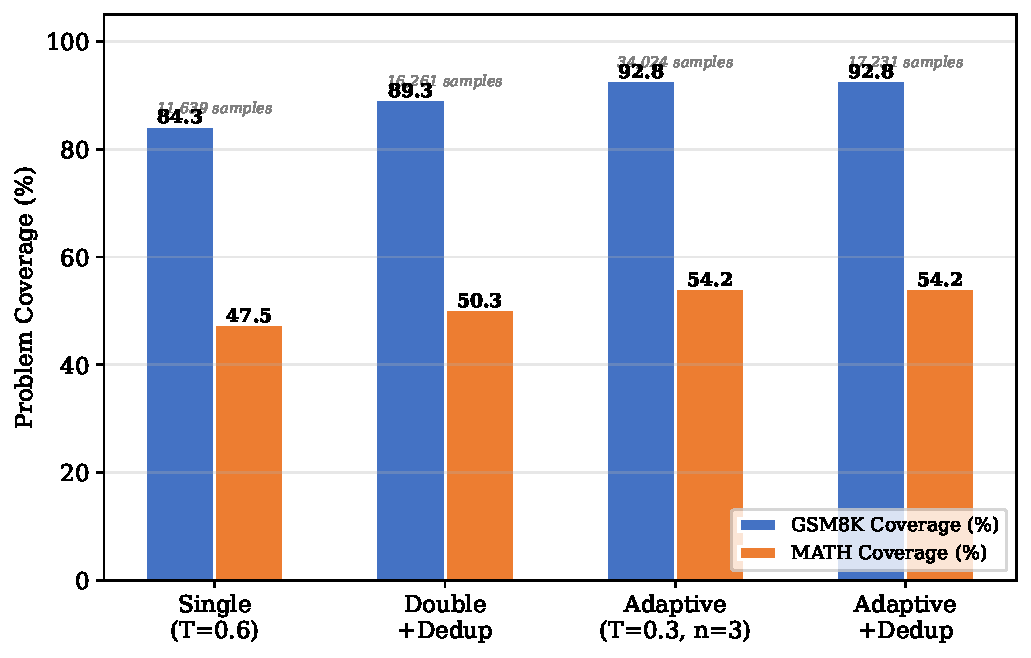
\includegraphics[width=0.85\textwidth]{figures/coverage_comparison.pdf}
    \caption{Training data coverage by strategy. Numbers above bars indicate total correct samples.}
    \label{fig:coverage}
\end{figure}

\subsection{Student Fine-tuning}

We fine-tuned Qwen2.5-0.5B-Instruct on each of the three training datasets (single-temperature, double-temperature, and adaptive), and subsequently fine-tuned Qwen2.5-0.5B base on the adaptive\_dedup dataset (17,231 samples). All runs used identical hyperparameters as described in Section~3.5 (3 epochs, effective batch size 16, $\text{lr}=2\times10^{-5}$, BF16, max 1,024 tokens, 5\% eval split). The best checkpoint per run was selected by lowest evaluation loss.

\subsection{Student Model Evaluation on Test Sets}

\subsubsection{Instruct Model Results}

To assess the effectiveness of our knowledge distillation pipeline, we first evaluated the three Instruct-based fine-tuned student models on the GSM8K (1,319 test samples) and MATH (1,250 test samples) benchmarks. Table~\ref{tab:student_eval_instruct} summarizes the overall accuracy.

\begin{table}[H]
\centering
\caption{Student model evaluation accuracy on GSM8K and MATH test sets (Instruct-based). The baseline is the pre-fine-tuned Qwen2.5-0.5B-Instruct evaluated zero-shot. Valid accuracy excludes samples with empty or unparseable answers.}
\label{tab:student_eval_instruct}
\begin{tabular}{lcccc}
\toprule
\textbf{Model} & \textbf{GSM8K} & \textbf{MATH} & \textbf{GSM8K (Valid)} & \textbf{MATH (Valid)} \\
\midrule
Baseline (Instruct, no fine-tune)  & 40.94\% & -- & 41.80\% & -- \\
\midrule
Single Temp ($T = 0.6$)     & 38.89\% & 19.76\% & 39.28\% & 20.05\% \\
Double Temp + Dedup          & 39.88\% & \textbf{20.24\%} & 40.34\% & \textbf{20.37\%} \\
Adaptive ($T = 0.3$, $n=3$)  & \textbf{41.55\%} & 19.04\% & \textbf{42.02\%} & 19.19\% \\
\bottomrule
\end{tabular}
\end{table}

The most striking result is that the non-fine-tuned baseline (40.94\%) \textit{outperforms} two of the three fine-tuned models on GSM8K. Only the adaptive strategy (41.55\%) surpasses the baseline, by a marginal 0.61 pp. This warrants careful analysis, as it challenges the assumption that CoT distillation uniformly improves student performance.

\subsubsection{The Distillation Tax: Why Fine-Tuning Can Hurt}

The underperformance of fine-tuned models relative to baseline on GSM8K reveals a fundamental challenge in knowledge distillation with instruction-tuned models: \textbf{distribution shift interference}. Qwen2.5-0.5B-Instruct already possesses non-trivial mathematical reasoning capability in its native concise style. Fine-tuning this model on CoT traces generated by DeepSeek-R1-Distill-Qwen-1.5B introduces a conflicting distribution:

\begin{enumerate}[leftmargin=*]
    \item \textbf{Reasoning style mismatch.} The Instruct model was tuned to produce concise, direct answers. DeepSeek-R1-Distill-Qwen-1.5B, in contrast, generates verbose chain-of-thought reasoning with extensive verification, self-reflection, and exhaustive enumeration. Forcing the student to adopt this foreign style causes interference with its native problem-solving heuristics.
    \item \textbf{Catastrophic interference at low data volumes.} With only 11,639 samples (single-temperature), the model partially overwrites its native reasoning patterns without fully acquiring the teacher's CoT style. The result is a 2.05 pp \textit{decrease} from baseline.
    \item \textbf{Recovery through data scale.} The double-temperature strategy (16,261 samples) reduces the gap to 1.06 pp below baseline, and the adaptive strategy (34,024 samples) finally surpasses baseline by 0.61 pp. However, the returns are diminishing: tripling the data yields only a 2.66 pp improvement, most of which merely recovers lost ground.
\end{enumerate}

The 2.66 pp gap between adaptive and single-temperature should thus be interpreted as adaptive \textit{recovering} 2.66 pp of the performance lost to distillation interference, rather than providing genuine improvement. The true gain over the non-fine-tuned baseline is at most 0.61 pp. This serves as a cautionary observation: for tasks where the student already has competence, distillation can be counterproductive unless sufficient data volume and diversity are provided to overcome the distribution shift.

\subsubsection{Base Model Results}

The Instruct-based results motivated our switch to the base model (Section~3.2). Table~\ref{tab:student_eval_base} presents the evaluation results for Qwen2.5-0.5B base before and after fine-tuning on the adaptive\_dedup dataset.

\begin{table}[H]
\centering
\caption{Evaluation results for Qwen2.5-0.5B base model on GSM8K and MATH. Baseline is zero-shot (no fine-tuning). Valid accuracy excludes samples with empty or unparseable answers.}
\label{tab:student_eval_base}
\begin{tabular}{lcccccc}
\toprule
\textbf{Model} & \textbf{GSM8K} & \textbf{MATH} & \textbf{GSM8K (V)} & \textbf{MATH (V)} & \textbf{Empty (G)} & \textbf{Empty (M)} \\
\midrule
Baseline (zero-shot)          & 13.80\% & 13.04\% & 33.27\% & 23.42\% & 58.0\% & 44.3\% \\
Base + Adaptive\_Dedup        & \textbf{42.76\%} & \textbf{23.28\%} & \textbf{43.62\%} & \textbf{24.15\%} & 1.2\% & 3.6\% \\
\bottomrule
\end{tabular}
\end{table}

The baseline base model achieves only 13.80\% accuracy on GSM8K and 13.04\% on MATH, with empty-answer rates of 58.0\% and 44.3\% respectively. A closer examination of the GSM8K baseline predictions reveals a deeper issue: 128 of 1,319 samples (9.7\%) exhibit \textbf{degenerative looping}, where the model falls into a repetitive token pattern-outputting the same token or short phrase hundreds of times . This degeneration behavior is characteristic of base models prompted beyond their capabilities, and accounts for a substantial portion of the empty-answer rate: looped outputs rarely contain extractable answers.

After fine-tuning on the adaptive\_dedup dataset, GSM8K accuracy improves to 42.76\% (+28.96 pp) and MATH to 23.28\% (+10.24 pp), while empty rates collapse from 58.0\%/44.3\% to 1.2\%/3.6\%. The MATH gain of 23.28\% is particularly significant: it exceeds the Instruct baseline (22.72\%) and all Instruct fine-tuned models (best: double-temperature, 20.24\%), marking the first time distillation produces positive MATH improvement over the unmodified model. This is in stark contrast to the Instruct-based results where every fine-tuned model underperformed the baseline on MATH (Section~4.4.1).

The dramatic reduction in empty outputs reflects more than just improved reasoning: the fine-tuned model has learned to produce properly formatted outputs with \texttt{\textbackslash{}boxed\{\}} markers, closely aligning with the teacher's CoT style. The format alignment is evident in the valid-answer rates: 98.8\% (GSM8K) and 96.4\% (MATH) of fine-tuned outputs contain extractable answers, compared to only 42.0\%/55.7\% for the zero-shot baseline. The fine-tuned model also exhibits virtually no degenerative looping, demonstrating that the CoT distillation process simultaneously teaches three capabilities: (1) mathematical reasoning itself, (2) output format discipline (\texttt{\textbackslash{}boxed\{\}} adherence), and (3) generation stability (prevention of repetitive token collapse). Unlike the Instruct model, the base model has no prior mathematical reasoning capability or format discipline, so the improvements are unambiguously attributable to the distillation process. Notably, the base+adaptive\_dedup model (42.76\% GSM8K, 23.28\% MATH) outperforms the best Instruct-based fine-tuned model (adaptive: 41.55\% GSM8K, double-temp: 20.24\% MATH), despite using half the training samples (17,231 vs.\ 34,024) and starting from a far weaker baseline (13.80\% vs.\ 40.94\% on GSM8K). This confirms that the switch to the base model was essential for valid measurement of distillation effectiveness, and that semantic deduplication preserves sufficient training signal quality while eliminating redundant samples.

\begin{figure}[H]
    \centering
    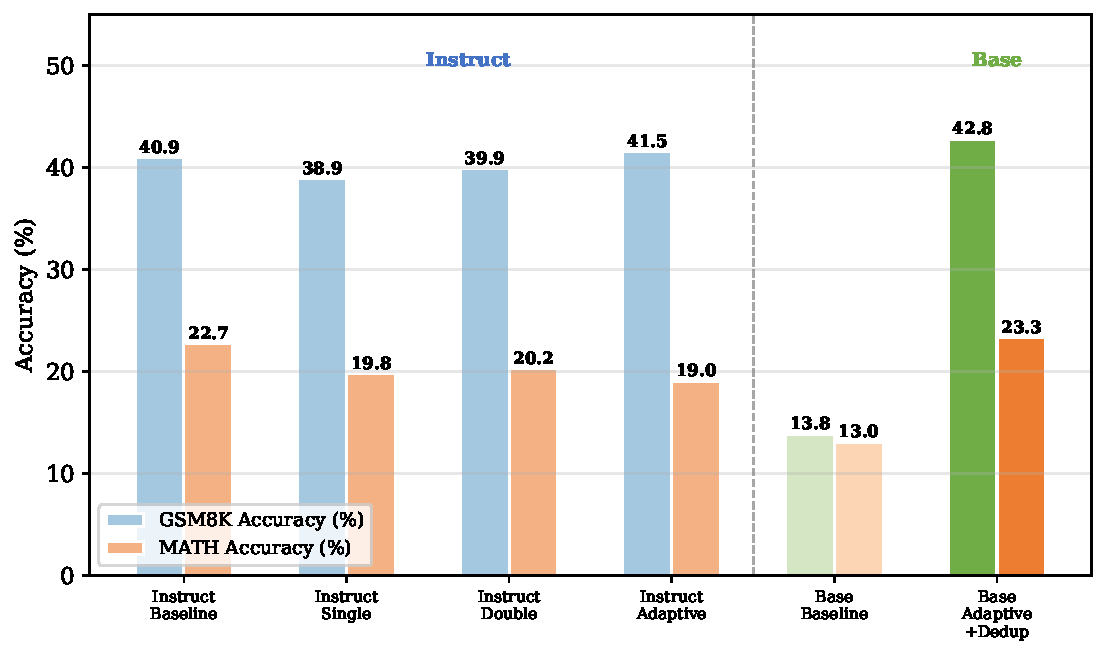
\includegraphics[width=0.9\textwidth]{figures/student_accuracy.pdf}
    \caption{Student model accuracy on GSM8K and MATH. The dashed line separates Instruct-based models (left) from Base models (right).}
    \label{fig:accuracy}
\end{figure}

\subsubsection{The Role of Semantic Deduplication and Multi-Temperature Diversity}

Two architectural decisions critically shape downstream performance: semantic deduplication and multi-temperature generation.

\textbf{Semantic Deduplication.} The double-temperature strategy achieves the best MATH accuracy among Instruct models (20.24\%), while the raw adaptive strategy-despite 2.09$\times$ more samples-underperforms on MATH (19.04\%). The adaptive\_dedup variant (Table~\ref{tab:comparison}) demonstrates deduplication's value: applying the 0.92 threshold reduces samples from 34,024 to 17,231 while preserving coverage identically (92.8\% GSM8K, 54.2\% MATH). The base model fine-tuned on this deduplicated dataset achieves 42.76\% GSM8K (+28.96 pp), outperforming the best Instruct model (41.55\%) with half the training data. This confirms that \textit{dataset size alone is a poor proxy for training signal quality}: deduplication removes near-duplicates that cause gradient imbalance and template overfitting without sacrificing problem coverage.

\textbf{Multi-Temperature Diversity.} The double-temperature strategy's high-temperature branch ($T = 0.9$) adds 374 GSM8K and 321 MATH problems not covered by single-temperature alone. These diverse answers survive deduplication because they differ meaningfully from the incorrect low-temperature outputs. In contrast, 70.7\% of adaptive's same-problem pairs at $T = 0.3$ are near-duplicates. The key insight is that \textit{inter-temperature diversity} (across $T$ values) substantially exceeds \textit{intra-temperature diversity} (multiple samples at fixed $T$). Applying this insight to the base model pipeline-combining adaptive deduplication with calibrated high-temperature resampling for uncertain problems-is a key direction for future work.

\subsubsection{Strategy Selection and Model Migration}

Based on the above analysis, we select \textbf{adaptive sampling with semantic deduplication} (adaptive\_dedup) as our recommended dataset construction strategy. This combines the best problem coverage (92.8\% GSM8K, 54.2\% MATH) with efficient sample density (1.3 samples per covered problem). The base model results validate this choice: adaptive\_dedup achieves 42.76\% GSM8K (+28.96 pp) and 23.28\% MATH (+10.24 pp), genuine distillation gains that exceed the best Instruct models (41.55\% GSM8K, 20.24\% MATH) despite using half the data. Base-model ablation experiments across all three strategies remain as future work to isolate the individual contributions of deduplication and multi-temperature generation.


\section{Conclusion}

We presented a study of knowledge distillation for mathematical reasoning, comparing three CoT sampling strategies. Key findings: (1) Problem coverage, not sample count, is the right metric-adaptive sampling achieves the highest coverage (92.8\% GSM8K, 54.2\% MATH), and semantic deduplication halves the dataset while preserving coverage identically. (2) A \textit{distillation tax} was observed with instruction-tuned models: fine-tuning on foreign-style CoT traces degrades the Instruct model's native reasoning, with only the largest dataset recovering above baseline (+0.61 pp). (3) Switching to a base student model eliminates this confound: fine-tuning on adaptive\_dedup improves GSM8K from 13.80\% to 42.76\% (+28.96 pp) and MATH from 13.04\% to 23.28\% (+10.24 pp), with empty rates collapsing from 58.0\%/44.3\% to 1.2\%/3.6\%. The MATH result exceeds both the Instruct baseline (22.72\%) and all Instruct fine-tuned models, marking the first positive distillation gain on MATH. The improvements reflect joint teaching of reasoning capability, output format discipline, and generation stability-all unambiguously attributable to distillation. (4) Multi-temperature generation meaningfully expands coverage-the high-temperature branch adds 374 GSM8K and 321 MATH problems-and inter-temperature diversity substantially exceeds intra-temperature diversity. (5) Log-probability-based confidence provides a zero-overhead alternative to self-consistency voting. We recommend adaptive sampling with semantic deduplication on a base student model as the most effective strategy for CoT distillation.

Several limitations of this study should be acknowledged. First, due to time constraints, we were unable to conduct full ablation experiments on the base model-comparing single-temperature, double-temperature, and adaptive strategies with and without deduplication-which limits the strength of our claims about the individual contributions of deduplication and adaptive sampling. The current evidence for these components comes primarily from Instruct-based experiments and dataset-level analysis; direct base-model ablation would provide more conclusive support. Second, the answer extraction pipeline relies on heuristic pattern matching (\texttt{\textbackslash{}boxed\{\}}, \texttt{**Answer:**} markers, and last-number fallback). This is particularly problematic for the base model baseline: the untuned model rarely produces \texttt{\textbackslash{}boxed\{\}} or \texttt{**Answer:**} markers, and the last-number fallback only activates when the generated text ends with a period-a condition violated by the 9.7\% of samples exhibiting degenerative looping (Section~4.4.3). Consequently, the 58.0\% empty-answer rate likely overstates the true failure rate, as correctly reasoned answers embedded in natural language or preceding a token-loop collapse go undetected by the extraction heuristics. Third, our analysis of CoT quality (Section~3.5) is based on surface-level pattern matching rather than semantic assessment of reasoning correctness; a CoT may be structurally well-formed yet contain logical errors that go undetected. Fourth, the teacher model does not always adhere to the system prompt instruction to place final answers in \texttt{\textbackslash{}boxed\{\}}: 8.1\%--13.5\% of training samples use alternative formats such as \texttt{**Answer:**} or plain text (Table~\ref{tab:cot_quality}). While these answers are correctly extracted by fallback mechanisms and included in training, they present inconsistent formatting to the student. A systematic post-processing step to reformat correct-but-misformatted teacher outputs into the canonical \texttt{\textbackslash{}boxed\{\}} style would improve training data consistency. Finally, all experiments use a single teacher–student architecture pair; the generalizability of our findings to other model families and scales remains to be tested.

\section{Future Work}

Several directions remain for future investigation:

\begin{enumerate}[leftmargin=*]
    \item \textbf{Adaptive sampling policy.} The current fixed threshold $\tau = -1.8$ failed to discriminate between confident and unconfident generations (Section~3.3.5). Two directions for improvement: (1) a static calibration approach that tunes $\tau$ via pilot-study analysis of log-probability distributions on a representative problem subset; and (2) a learned sampling policy that conditions temperature and sampling count on richer state features-problem embedding, number of existing samples, log-probability statistics of current answers-trained via reinforcement learning to balance coverage against sampling cost. The latter would transform the adaptive strategy from a heuristic pipeline into an optimized data acquisition process.
    \item \textbf{CoT quality scoring and filtering.} Currently only answer correctness is used to filter training samples. However, some CoT traces produce correct final answers despite containing flawed reasoning, self-correction loops, or excessive repetition. Developing an automated CoT quality scoring mechanism-independent of answer correctness-would allow filtering of samples where the reasoning process itself is of low quality, even if the final answer happens to be correct.
    \item \textbf{CoT post-processing.} The quality analysis in Section~3.5 identified self-correction patterns ($\sim$0.4\% of samples) and highly repetitive traces ($\sim$0.2\%) that may negatively impact student training. Systematic detection and removal or repair of these patterns-for instance, collapsing repeated enumeration loops into concise summaries, or stripping mid-reasoning error-correction segments-could improve training data quality without reducing problem coverage.
    \item \textbf{Iterative distillation.} Multiple rounds of student-generated CoT refinement, where the fine-tuned student generates its own reasoning traces that are filtered and used for subsequent training, potentially enabling the student to progressively surpass the teacher.
    \item \textbf{Error-correction distillation.} Targeted augmentation using problems where the student answers incorrectly but the teacher answers correctly. These error-specific samples provide focused corrective supervision. The teacher could also generate new, similar problems targeting the same reasoning patterns, reinforcing weak skills without memorization.
    \item \textbf{Reinforcement learning for reasoning (GRPO).} Applying Group Relative Policy Optimization (GRPO) after SFT: the student samples multiple reasoning paths per problem, rewarded on correctness and format, and updated via relative group-wise advantage. GRPO requires no critic network, making it memory-efficient for the 0.5B model. SFT $\rightarrow$ GRPO offers a viable path for the student to surpass the teacher.
\end{enumerate}


\section*{Acknowledgements}

\medskip


\bibliographystyle{plain}

\bibliography{ref}


\end{document}
